\section{Datenverarbeitung}
\label{sec:Datenverarbeitung}
Der \ac{Raspi} ist für die Datenverarbeitung zuständig, einerseits empfängt er die Daten von den verschiedenen Sensoren, andererseits schreibt er alle gesammelten Messwerte auf die microSD-Karte. Diese Operationen werden alle von einem Python-Programm erledigt. Dieses Programm wird mithilfe des init-Systems \glqq systemd\grqq\ (\url{https://systemd.io/}) automatisch gestartet, wenn der Raspberry Pi startet. Wenn der Raspberry Pi mit Spannung versorgt wird, (siehe Sektion \ref{subsec:elekSupply}) startet der Einplatinencomputer automatisch. Ist der Startvorgang abgeschlossen, leuchtet die eingebaute \ac{LED} in Rot auf. Um das automatische Starten des Programmes zu deaktivieren, kann der Befehl \verb|sudo systemctl disable automotion.service| verwendet werden. Um das automatische Starten zu reaktivieren, kann der Befehl \verb|sudo systemctl enable automotion.service| verwendet werden.
\subsection{Datenaufzeichnungsmodus}
\label{subsec:Datenaufzeichnungsmodus}
Mithilfe eines Tasters kann zwischen zwei Modi umgeschalten werden, einer davon ist der Datenaufzeichnungsmodus, welcher durch die Farbe Blau der eingebauten \ac{LED} indiziert wird. In diesem Modus werden die Daten von allen verbauten Sensoren gesammelt und anschließend auf den Speicher des \ac{Raspi} geschrieben. Jedes Mal, wenn das Programm gestartet wird, wird eine neue Textdatei mithilfe der von der in Sektion \ref{subsubsec:tLibOs} beschriebenen Python-Bibliothek \glqq os\grqq\ bereitgestellten Funktion \verb|open()| erstellt. Das von dieser Funktion zurückgegebene Objekt wird dann verwendet, um die erstellte Datei zu bearbeiten. Die gesammelten Daten werden von den jeweiligen Sensorimplementationen bereitgestellt und in einem vorgegebenen Takt (standardmäßig einmal pro Sekunde) als Datensatz in eine neue Zeile in die Datei geschrieben. Um die Daten von allen Sensoren simultan auszulesen und für die Aufzeichnung bereitzustellen, wird unter anderem die Python-Bibliothek \glqq multiprocessing\grqq\ verwendet. Diese Bibliothek ermöglicht es, verschiedene Funktionen simultan (parallel) auf dem Raspberry Pi auszuführen, das Ressourcenmanagement übernimmt dabei der Linux-Kernel von Raspberry Pi OS. Dieses Multiprocessing wird benötigt, weil die verschiedenen Sensoren unterschiedliche Zeitverzögerungen benötigen. Ein Beispiel dafür ist die \ac{IMU}, welche für die Sensorfusion Delays benötigt. Jeder Datensatz besteht aus der Zeit der Datenaufnahme, der Orientierung, den Beschleunigungen, der Umgebungstemperatur, den Drehzahlen, der Geschwindigkeit und den Koordinaten. Die jeweiligen Werte sind voneinander mit Kommas getrennt, um die Kompatibilität mit Tabellenkalkulationsprogrammen wie Microsoft Excel oder LibreOffice Calc zu gewährleisten.
\subsection{Datenübertragungsmodus}
\label{subsec:Datenübertragungsmodus}
Der andere zur Verfügung stehende Modus ist der der Datenübertragung auf ein \ac{USB} Wechselmedium. Dieser Modus ist der Modus, in dem der \ac{Raspi} sich befindet, nachdem er gestartet wurde, er wird durch die Farbe Rot der eingebauten \ac{LED} signalisiert. In diesem Modus überprüft der Raspberry Pi jede Sekunde, ob an dem Einhängepunkt \verb|/media/usb0| ein Gerät erscheint. Das Einhängen des Datenträgers übernimmt das Paket \glqq usbmount\grqq , welches am Raspberry Pi mit dem Befehl \verb|sudo apt install usbmount| installiert werden kann. Zusätzlich zur Installation des Paketes muss noch in der Datei \verb|/lib/systemd/system/systemd-udevd.service| die Option \verb|PrivateMounts=no| gesetzt werden. Sollte ein Datenträger eingehängt werden, werden alle erstellten Dateien in 100 Millisekunden-Abständen mithilfe der von der in Sektion \ref{subsubsec:tShutil} beschriebenen Python-Bibliothek \glqq shutil\grqq\ bereitgestellten Funktion \verb|copy()| in das Stammverzeichnis des \ac{USB}-Wechselmediums kopiert. Um einen erfolgreichen Kopiervorgang zu signalisieren, blinkt die eingebaute \ac{LED} pro kopierter Datei einmal Grün. Dafür sollte der Datenträger mit einem Dateisystem wie \ac{NTFS} oder \ac{FAT} formatiert sein, welches sowohl unter Linux als auch unter Microsoft Windows eingehängt werden kann. Das Programm kann manuell mit dem Befehl \verb|sudo python3 main.py| ausgeführt werden. Das \glqq sudo\grqq\ ist hierbei dafür zuständig, dass das Programm mit Administratorberechtigungen (root-Berechtigungen) ausgeführt wird. Diese werden benötigt, da das Paket \glqq usbmount\grqq\ Datenträger standardmäßig nur als read-only für normale Nutzer einhängt. Um auf den Datenträger schreiben zu können werden deswegen root-Berechtigungen benötigt.
\subsection{Live-Datenausgabe}
\label{subsec:LiveDatenausgabe}
Zusätzlich zur Speicherung auf dem Raspberry Pi werden die Daten live in die Befehlszeile ausgegeben, in der das Programm ausgeführt wird. Somit können die Daten live auf einem Computer oder Smartphone ausgelesen werden, solange sich das Auto in Reichweite eines \ac{WLAN} Signals befindet und sich die Geräte im selben Netzwerk befinden. Um diese live-Übertragung zu verwenden, kann das Gerät, auf dem die Daten angezeigt werden sollen via \ac{SSH} mit dem Raspberry Pi verbunden werden und dann das Programm ausführen. Diese Art der Datenausgabe kann in Abbildung \ref{fig:liveDaten} gesehen werden.
\begin{figure}[h]
\centering
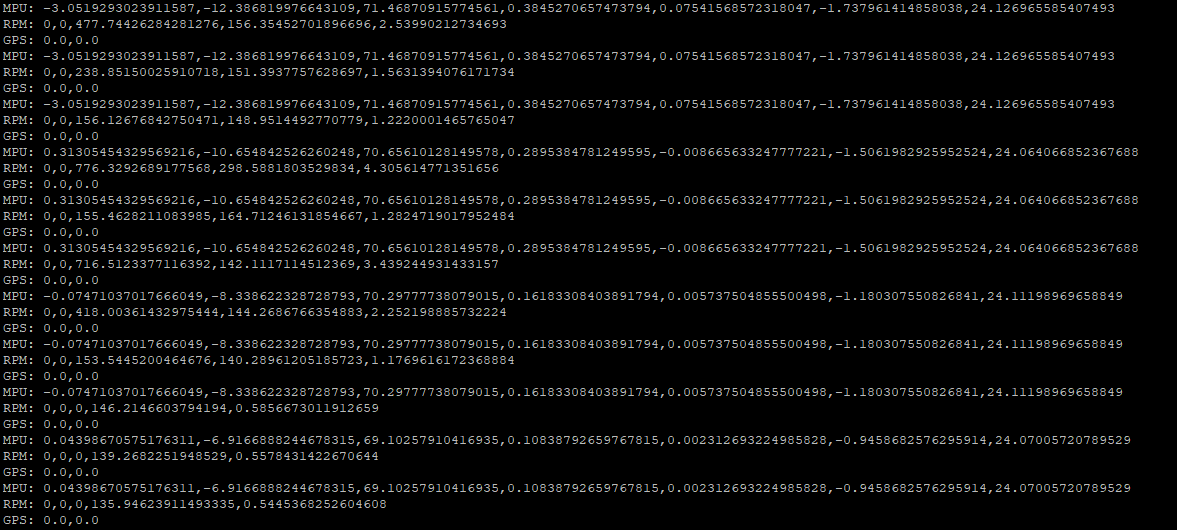
\includegraphics[scale=0.36]{LiveDaten.png}
\caption{Live-Datenübertragung}
\label{fig:liveDaten}
\end{figure}